% This file was created by matplotlib2tikz v0.6.14.
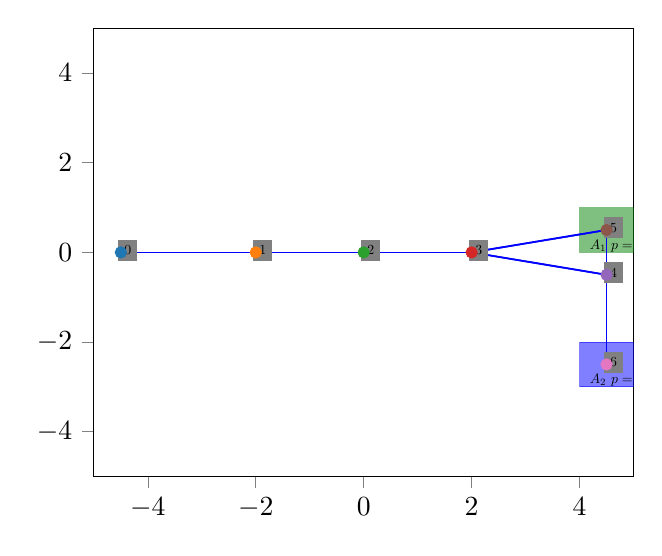
\begin{tikzpicture}

\definecolor{color1}{rgb}{1,0.498039215686275,0.0549019607843137}
\definecolor{color0}{rgb}{0.12156862745098,0.466666666666667,0.705882352941177}
\definecolor{color3}{rgb}{0.83921568627451,0.152941176470588,0.156862745098039}
\definecolor{color2}{rgb}{0.172549019607843,0.627450980392157,0.172549019607843}
\definecolor{color5}{rgb}{0.549019607843137,0.337254901960784,0.294117647058824}
\definecolor{color4}{rgb}{0.580392156862745,0.403921568627451,0.741176470588235}
\definecolor{color6}{rgb}{0.890196078431372,0.466666666666667,0.76078431372549}

\begin{axis}[
xmin=-5, xmax=5,
ymin=-5, ymax=5,
tick align=outside,
tick pos=left,
x grid style={lightgray!92.02614379084967!black},
y grid style={lightgray!92.02614379084967!black}
]
\addplot [only marks, draw=color0, fill=color0, colormap/viridis, visualization depends on={\thisrow{sizedata} \as\perpointmarksize}, scatter/@pre marker code/.append style={/tikz/mark size=\perpointmarksize}]
table{%
x                      y                      sizedata
-4.500000000000000e+00 +0.000000000000000e+00 +3.385137501286538e+00
};
\addplot [only marks, draw=color1, fill=color1, colormap/viridis, visualization depends on={\thisrow{sizedata} \as\perpointmarksize}, scatter/@pre marker code/.append style={/tikz/mark size=\perpointmarksize}]
table{%
x                      y                      sizedata
-2.000000000000000e+00 +0.000000000000000e+00 +3.385137501286538e+00
};
\addplot [only marks, draw=color2, fill=color2, colormap/viridis, visualization depends on={\thisrow{sizedata} \as\perpointmarksize}, scatter/@pre marker code/.append style={/tikz/mark size=\perpointmarksize}]
table{%
x                      y                      sizedata
+0.000000000000000e+00 +0.000000000000000e+00 +3.385137501286538e+00
};
\addplot [only marks, draw=color3, fill=color3, colormap/viridis, visualization depends on={\thisrow{sizedata} \as\perpointmarksize}, scatter/@pre marker code/.append style={/tikz/mark size=\perpointmarksize}]
table{%
x                      y                      sizedata
+2.000000000000000e+00 +0.000000000000000e+00 +3.385137501286538e+00
};
\addplot [only marks, draw=color4, fill=color4, colormap/viridis, visualization depends on={\thisrow{sizedata} \as\perpointmarksize}, scatter/@pre marker code/.append style={/tikz/mark size=\perpointmarksize}]
table{%
x                      y                      sizedata
+4.500000000000000e+00 -5.000000000000000e-01 +3.385137501286538e+00
};
\addplot [only marks, draw=color5, fill=color5, colormap/viridis, visualization depends on={\thisrow{sizedata} \as\perpointmarksize}, scatter/@pre marker code/.append style={/tikz/mark size=\perpointmarksize}]
table{%
x                      y                      sizedata
+4.500000000000000e+00 +5.000000000000000e-01 +3.385137501286538e+00
};
\addplot [only marks, draw=color6, fill=color6, colormap/viridis, visualization depends on={\thisrow{sizedata} \as\perpointmarksize}, scatter/@pre marker code/.append style={/tikz/mark size=\perpointmarksize}]
table{%
x                      y                      sizedata
+4.500000000000000e+00 -2.500000000000000e+00 +3.385137501286538e+00
};
\path [draw=green!50.19607843137255!black, fill=green!50.19607843137255!black, opacity=0.5] (axis cs:5,-9.86076131526264e-31)
--(axis cs:5,1)
--(axis cs:4,1)
--(axis cs:4,-7.88860905221011e-31)
--cycle;

\path [draw=blue, fill=blue, opacity=0.5] (axis cs:5,-3)
--(axis cs:5,-2)
--(axis cs:4,-2)
--(axis cs:4,-3)
--cycle;

\addplot [semithick, blue, forget plot]
table {%
-4.5 0
-2 0
};
\addplot [semithick, blue, forget plot]
table {%
-2 0
-4.5 0
};
\addplot [semithick, blue, forget plot]
table {%
-2 0
0 0
};
\addplot [semithick, blue, forget plot]
table {%
0 0
-2 0
};
\addplot [semithick, blue, forget plot]
table {%
0 0
2 0
};
\addplot [semithick, blue, forget plot]
table {%
2 0
0 0
};
\addplot [semithick, blue, forget plot]
table {%
2 0
4.5 -0.5
};
\addplot [semithick, blue, forget plot]
table {%
2 0
4.5 0.5
};
\addplot [semithick, blue, forget plot]
table {%
4.5 -0.5
2 0
};
\addplot [semithick, blue, forget plot]
table {%
4.5 -0.5
4.5 0.5
};
\addplot [semithick, blue, forget plot]
table {%
4.5 -0.5
4.5 -2.5
};
\addplot [semithick, blue, forget plot]
table {%
4.5 0.5
2 0
};
\addplot [semithick, blue, forget plot]
table {%
4.5 0.5
4.5 -0.5
};
\addplot [semithick, blue, forget plot]
table {%
4.5 -2.5
4.5 -0.5
};
\node at (axis cs:-4.54,-0.05)[
  scale=0.5,
  fill=lightgray!66.92810457516339!black,
  draw=lightgray!66.92810457516339!black,
  line width=0.4pt,
  inner sep=4pt,
  anchor=base west,
  text=black,
  rotate=0.0
]{ 0};
\node at (axis cs:-2.04,-0.05)[
  scale=0.5,
  fill=lightgray!66.92810457516339!black,
  draw=lightgray!66.92810457516339!black,
  line width=0.4pt,
  inner sep=4pt,
  anchor=base west,
  text=black,
  rotate=0.0
]{ 1};
\node at (axis cs:-0.04,-0.05)[
  scale=0.5,
  fill=lightgray!66.92810457516339!black,
  draw=lightgray!66.92810457516339!black,
  line width=0.4pt,
  inner sep=4pt,
  anchor=base west,
  text=black,
  rotate=0.0
]{ 2};
\node at (axis cs:1.96,-0.05)[
  scale=0.5,
  fill=lightgray!66.92810457516339!black,
  draw=lightgray!66.92810457516339!black,
  line width=0.4pt,
  inner sep=4pt,
  anchor=base west,
  text=black,
  rotate=0.0
]{ 3};
\node at (axis cs:4.46,-0.55)[
  scale=0.5,
  fill=lightgray!66.92810457516339!black,
  draw=lightgray!66.92810457516339!black,
  line width=0.4pt,
  inner sep=4pt,
  anchor=base west,
  text=black,
  rotate=0.0
]{ 4};
\node at (axis cs:4.46,0.45)[
  scale=0.5,
  fill=lightgray!66.92810457516339!black,
  draw=lightgray!66.92810457516339!black,
  line width=0.4pt,
  inner sep=4pt,
  anchor=base west,
  text=black,
  rotate=0.0
]{ 5};
\node at (axis cs:4.46,-2.55)[
  scale=0.5,
  fill=lightgray!66.92810457516339!black,
  draw=lightgray!66.92810457516339!black,
  line width=0.4pt,
  inner sep=4pt,
  anchor=base west,
  text=black,
  rotate=0.0
]{ 6};
\node at (axis cs:4.1,0.0700000000000001)[
  scale=0.5,
  anchor=base west,
  text=black,
  rotate=0.0,
  align=left
]{ $A_1$
$p=0.9$};
\node at (axis cs:4.1,-2.93)[
  scale=0.5,
  anchor=base west,
  text=black,
  rotate=0.0,
  align=left
]{ $A_2$
$p=0.3$};
\end{axis}

\end{tikzpicture}